\section{Prospects for integrated array tomography}
\label{sec:5.1_valorisation}

This thesis presents a novel workflow for three-dimensional correlative light and electron microscopy (3D CLEM) in the form of integrated array tomography. The method involves correlative imaging of and volume reconstruction from serial sections of biological tissue using an integrated fluorescence and electron microscope, which offers several advantages over alternative approaches for 3D CLEM.

% \setlist{nolistsep}
\begin{enumerate}[label=(\Roman*)]
    \item Semi-automated imaging and fully-automated registration facilitate the correlative acquisition of large numbers of serial sections. We have demonstrated the scalability of our method to 64 sections of zebrafish pancreas in which the only limitation was on the number of serial sections that were prepared (Chapter \ref{chap:3}). Additionally, the correlative reconstruction routine supports the alignment of an arbitrarily large number of sections.
    \item \textit{In-situ} targeting of ROIs expedites throughput by limiting imaging volumes to those regions expressed by fluorescence. In practice we have experienced tenfold decreases in imaging volume with corresponding reductions to acquisition times and dataset sizes (Chapter \ref{chap:3}).
    \item Because the specimen is simultaneously prepared for both FM and EM, the reconstructed volumes of correlative data have matching axial resolution. This means that the fluorescence data does not have to be projected or interpolated in $z$ as is the case with certain sequential CLEM approaches. Furthermore, specimen warping and shrinkage between imaging modalities, which might otherwise occur in conventional array tomography methods, is prevented due to the absence of intermediate sample preparation.
    \item Precise overlay of biological molecules and structural context at high resolution is achievable in all three dimensions. We have demonstrated sub-\SI{100}{\nano\meter} typical overlay accuracy and worst-case-scenario misalignment of ${\sim}$\SI{1}{\micro\meter} (Chapter \ref{chap:3}).
    \item Array tomography allows for re-evaluation of sections, if necessary, as opposed to serial blockface (SBF-SEM) or focused ion beam (FIB-SEM) techniques in which the specimen is destroyed as it is imaged.
\end{enumerate}

While the method has its advantages, it is not, of course, without its limitations. Chief among them is the manual intervention needed for certain navigation and focusing tasks. Although the ability to detect regions of interest on-the-fly based on fluorescence is one of the main benefits of integrated array tomography, these regions must still be navigated to manually. To further automate the workflow, ROI positions for each section could be extrapolated based on an initial selection, as in \textcite{gabarre2021workflow}. Slight variations in section shape can be accounted for by a geometrical transformation of each serial section to the reference section from which the ROI was initially selected. An alternative approach for fully automated ROI detection and navigation involves recognition of the fluorescent markers of interest based on artificial intelligence (AI). \textcite{delpiano2018automated} investigated this approach for the automated detection of fluorescent cells, finding that current state-of-the-art machine learning techniques required significant quantities of ground truth training data as well as postprocessing for separating merged cells. Thus, while fully automated AI-based approaches for ROI detection may not yet be suitable, opportunities for extending automated navigation do exist.

The other component of the workflow that stands to benefit most from automation are the EM and FM focusing routines. Effort has been invested in developing an autofocus procedure for the fluorescence microscope (Appendix \ref{app:A}), which involved analyzing the performance of several dozen focus metrics. The results were ultimately incorporated into the autofocus routine implemented in the integrated microscope control software, Odemis. Developing an EM autofocus routine has been a more complex task as it requires access to proprietary software for controlling the lens voltages. With the development of FAST-EM \cite{fermie2021high}, access to these controls has become available through an extension to Odemis. The potential for fully automated focus routines is therefore in place, however, questions surrounding the robustness of these routines remain. Therefore, the choice was made to forgo autofocusing routines during large-scale acquisitions to prevent the possibility of a failure compromising subsequent acquisitions.

Many of the sub-routines involved in integrated array tomography have been fully automated (Figure \ref{fig:5.1_workflow}). This is particularly true of the alignment and reconstruction procedures, which are executed through a series of interactive jupyter notebooks that have been made publicly available.\footnote{\href{https://github.com/hoogenboom-group/iCAT-workflow}{https://github.com/hoogenboom-group/iCAT-workflow}} The section detection phase is similarly guided by a series of jupyter notebooks that perform the serial section segmentation and tile mapping (partitioning the ROI into low- and high-magnification image tiles) sub-routines.\footnote{\href{https://github.com/hoogenboom-group/secdetect}{https://github.com/hoogenboom-group/secdetect}} Note that the segmentation step is denoted as semi-automatic in Figure \ref{fig:5.1_workflow} since connected ribbons of serial sections often require manual correction to obtain an optimal instance segmentation. Software for acquiring grids of image tiles (including the CL-spot alignment during low-magnification CLEM) are available as a plugin in Odemis,\footnote{\href{https://github.com/delmic/odemis}{https://github.com/delmic/odemis}} which is fully open-source. This level of automation should in principle enable anyone with familiarity in fluorescence and electron microscopy as well as programming experience in Python to follow the integrated array tomography workflow with relative ease.

% Figure 5.1 (workflow)
% ---------------------
\begin{figure}[!tb]
    \centering
    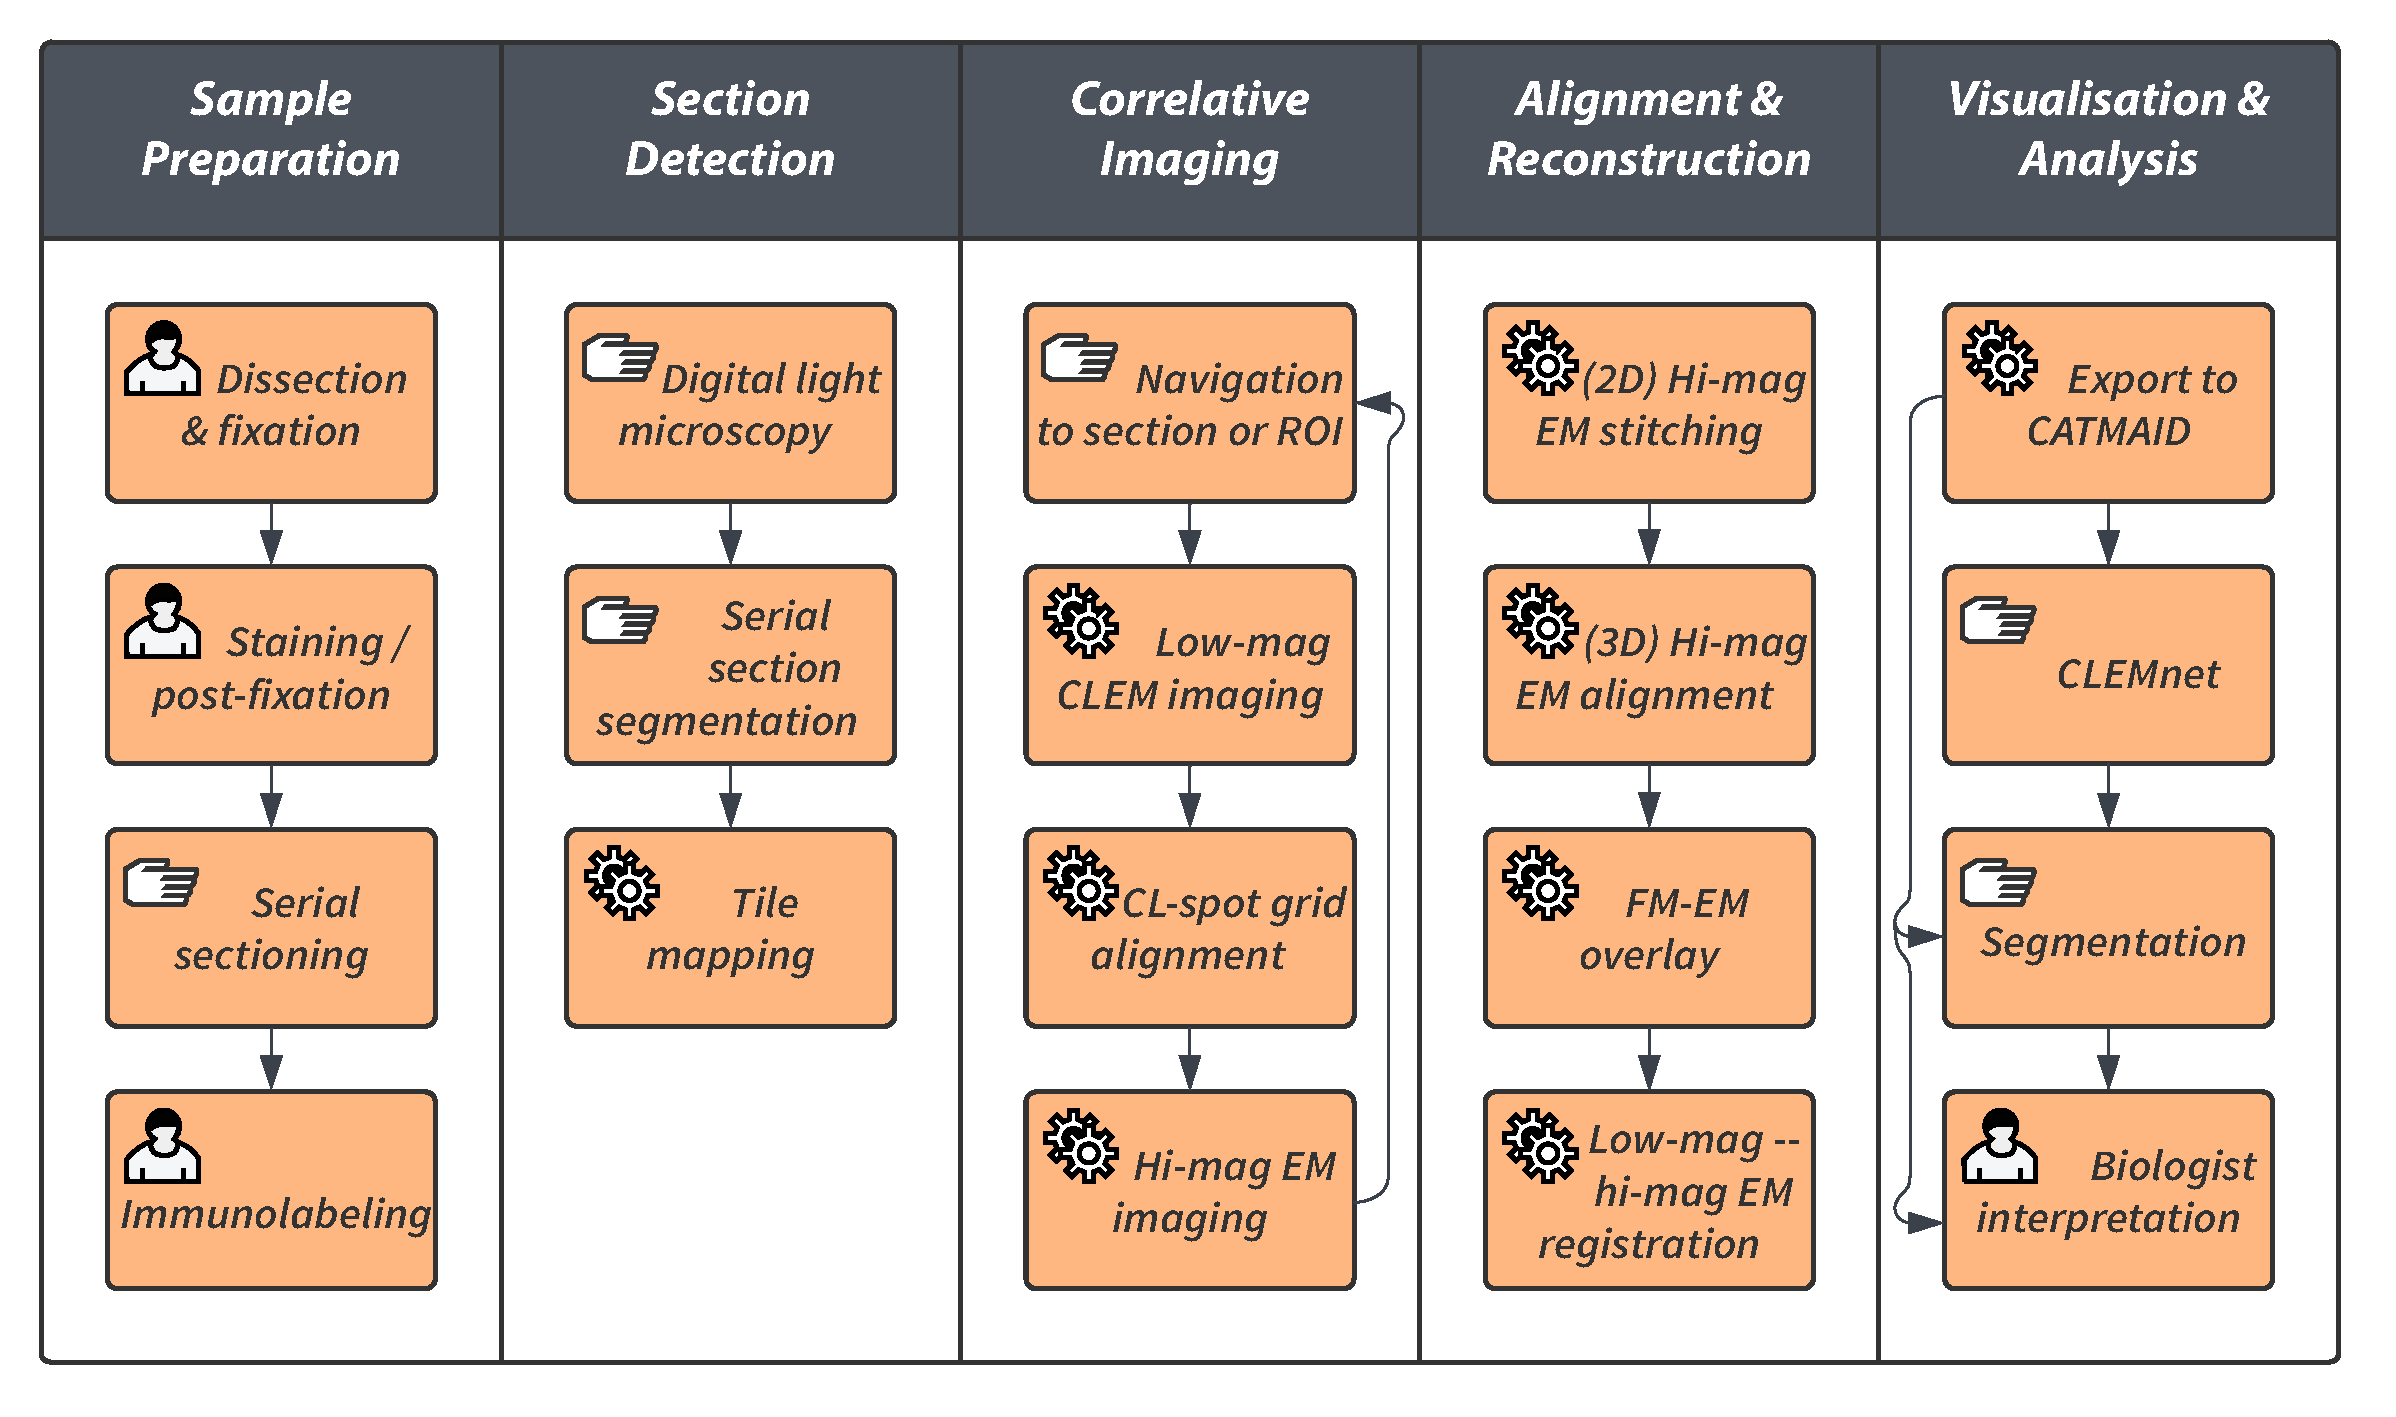
\includegraphics[width=\linewidth]{chapter-5/figures_PDF/fig5-1_workflow.pdf}
    \caption{Workflow diagram for integrated array tomography. Icons represent the extent to which each subroutine is automated: human -- fully manual, hand -- semi-automated or human-assisted, gears -- fully automated. Note that a sub-routine may still be considered fully automated even if it might benefit from further automation (e.g. implementing autofocus within high-magnification EM imaging).}
    \label{fig:5.1_workflow}
\end{figure}

Challenges pertaining to sample preparation were described in Section \ref{sec:3.4_discussion}. In short, fluorescent probes, such as fluorescent proteins, are generally incompatible with conventional fixation and staining procedures used for EM. Despite efforts towards developing probes for retaining fluorescence post-embedding \cite{watanabe2011protein, kukulski2011correlated, peddie2014correlative}, compromises between the strength of the fluorescence and the quality of the ultrastructure remain unavoidable. These compromises are made more difficult by conducting fluorescence imaging in high vacuum conditions where intensities are expected to be lower as fluorescent probes are typically optimized for (if not dependent on) aqueous environments \cite{peddie2014correlative}.

Finally, fluorescence preservation or post-embedding relabeling of genetic fluorophores may facilitate linking ultrastructural observations to live, intravital fluorescence microscopy. Prior to array tomography, photoactivatable probes could be used to mark where cells can be assessed for function. These markers could then be activated as part of the integrated workflow, thus linking the ultrastructural data to not only fluorescence expression but also to function and development \cite{collinson2017correlating}. If combined with advances in automation, this could lead towards the development of dedicated integrated CLEM instruments with complete and fully automated workflows for high-throughput and high-yield volume CLEM.
